\section{JBIMulti2}
\label{sec:jbimulti2}  

A multi-tenant management system must fulfill several requirements, such as data and performance isolation between tenants and users, authentication, specification of different user roles, resources usage monitoring, etc. In a \ac{JBI} environment, endpoint and routing configurations files are packed in \ac{SU}s, and the latter in \ac{SA}s for deployment. However, there is a lack of user-specific data during deployment. Muhler solves this problem in JBIMulti2 by injecting tenant context in the \ac{SA} packages, making them tenant-aware \cite{Muhler2012}. 

\begin{figure}[htb]
	\centering
		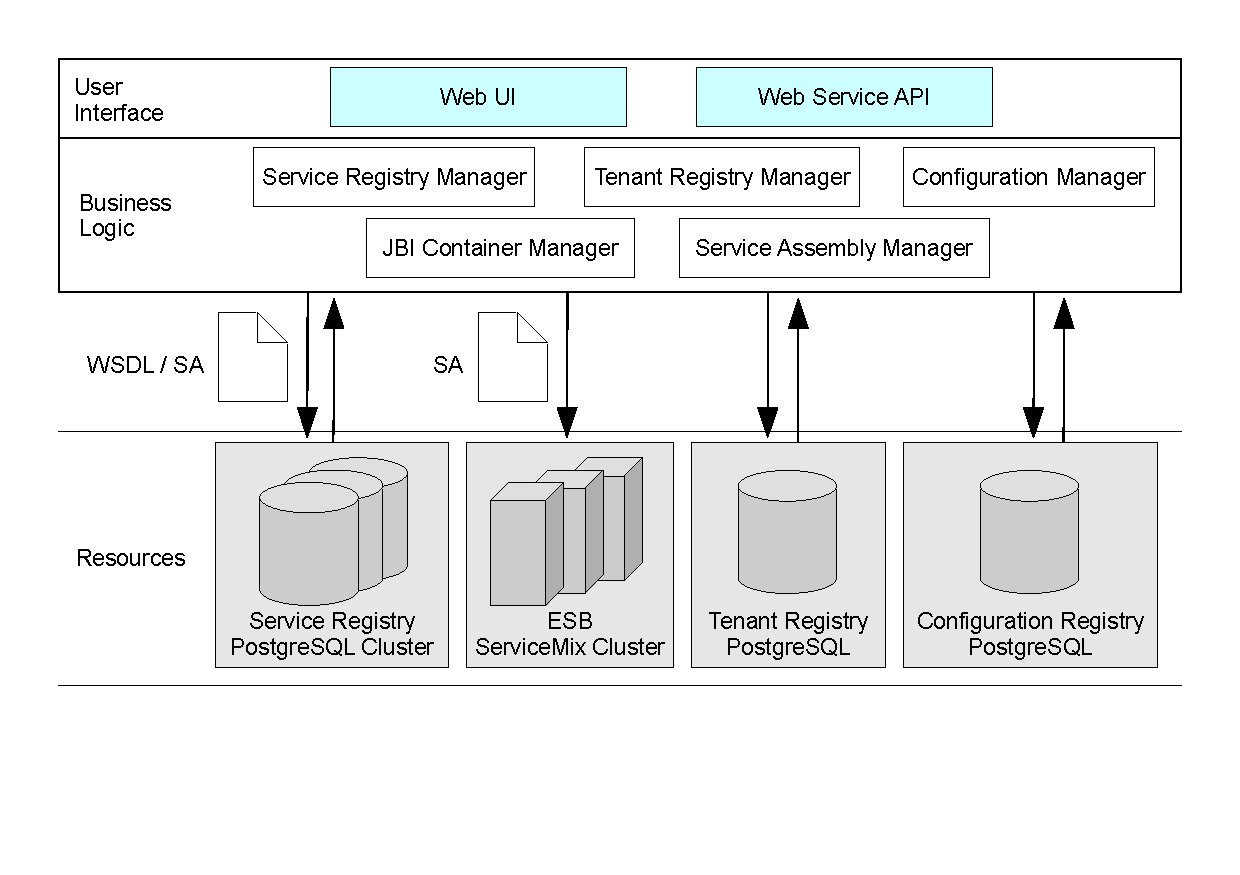
\includegraphics[clip, scale=0.5]{./gfx/systemoverview_jbimulti2.pdf}
	\caption[JBIMulti2 System Overview]{JBIMulti2 System Overview \cite{Muhler2012}} 
	\label{fig:jbimulti2}
\end{figure}

The architecture of the JBIMulti2 system is represented in Figure \ref{fig:jbimulti2}. We can distinguish two main parts in the system: business logic and resources. JBIMulti2 uses three registries for storing configuration and management data. When a tenant (or a tenant user) is registered, an unique identification number is given to them and stored in the Tenant Registry. Both Tenant Registry and Service Registry are designed for storing data of more than one deployed application. The former for storing tenant information and the latter for providing a dynamic service discovery functionality between the different applications accessed through the \ac{ESB}. The Configuration Registry is the key of the tenant isolation requirement of the system. Each of the stored tables are indexed by the tenant id  and user id value. In this thesis we need tenant information during runtime. We reuse and extend the databases schemas produced by Muhler, specifically the Service Registry.

The system provides a user interface for accessing the application's business logic. Through the business logic, the management of tenants can be done by the system administrator or the management of tenant's users can be done by the tenants. Furthermore, when deploying the different tenant's endpoint configurations packed in \ac{SA}s, the system first makes modifications in the zip file for adding tenant context information and then communicates with the Apache ServiceMix instance by using a \ac{JMS} Topic to which all the ServiceMix instances are subscribed to. The \ac{JMS} management service in ServiceMix deploys the received \ac{SA} injected in the received \ac{JMS} message using the administration functionalities provided in ServiceMix. The communication between the business layer and the ServiceMix instance is unidirectional. When successful deployment, the endpoint is reachable by the tenant. When an error occur during deployment, an unprocessed management message is posted in a dead letter queue.

JBIMulti2 requires the previous installation of components, e.g. JOnAS server, PostgreSQL, etc. The initialization of the application is described in both Chapter \ref{chap:validationevaluation} and in the JBIMulti2 setup document \cite{JBIMulti2Man}.